\documentclass[12pt,ngerman]{beamer}
\usepackage[utf8]{inputenc}
\usepackage[T1]{fontenc}
\usepackage{booktabs}
\usepackage{babel}
\usepackage{graphicx}
\usepackage{csquotes}
\usepackage{xcolor}
\usepackage[]{listings} 
 
\usepackage[sfdefault]{plex-sans}
\usetheme[progressbar=frametitle]{metropolis}           % Use metropolis theme
 
\title{E-Mail Handling with Python}
\date{\today}
\author{Dr. Uwe Ziegenhagen}
\institute{www.uweziegenhagen.de}
 
\makeatletter
\setlength{\metropolis@titleseparator@linewidth}{1pt}
\setlength{\metropolis@progressonsectionpage@linewidth}{1pt}
\setlength{\metropolis@progressinheadfoot@linewidth}{1pt}
\makeatother
 
\begin{document}
 
\begin{frame}
	 \maketitle
\end{frame}
 
\begin{frame}
\frametitle{Introduction}
\framesubtitle{~}
 
\begin{itemize}
\item I am Vice-President of Dante e.V., the German \LaTeX\  society
\item My job: send e-mails to new members and manage mailing lists w.r.t. SPAM
\item Automating these two tasks with Python has high ROI (return-on-investment)
\end{itemize}


\begin{center}
https://github.com/UweZiegenhagen/E-Mail-Handling-in-Python
\end{center}

\end{frame}

\begin{frame}

\section{Handling E-Mails}

\end{frame}


\begin{frame}
\frametitle{Online Form at www.dante.de}

\begin{center}
\fbox{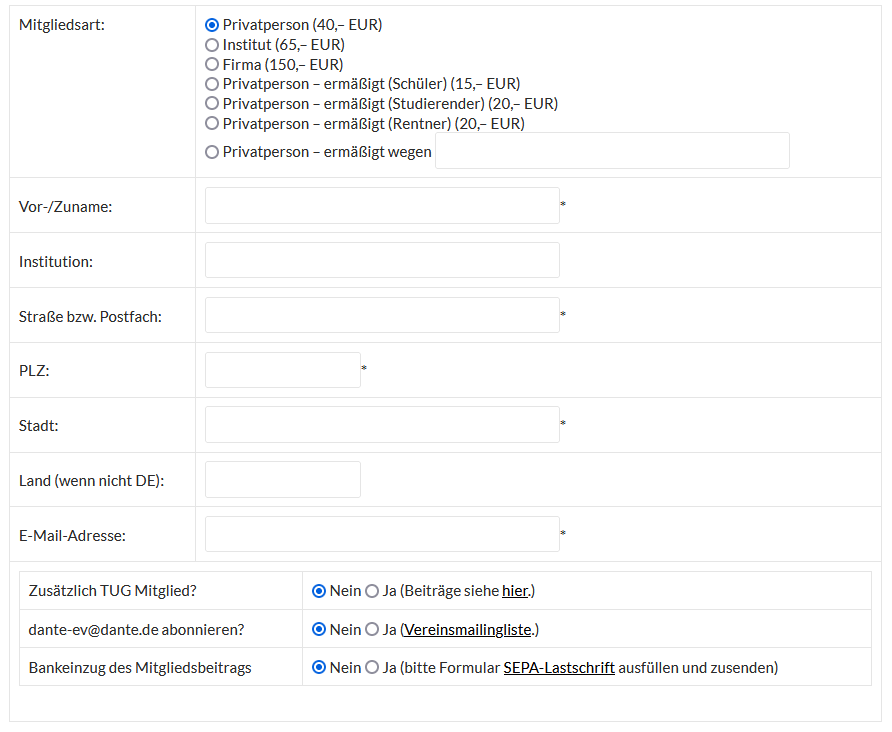
\includegraphics[width=0.8\textwidth]{onlineform}}
\end{center}

\end{frame}

\begin{frame}
\frametitle{Online Form at www.dante.de}

\begin{center}
\fbox{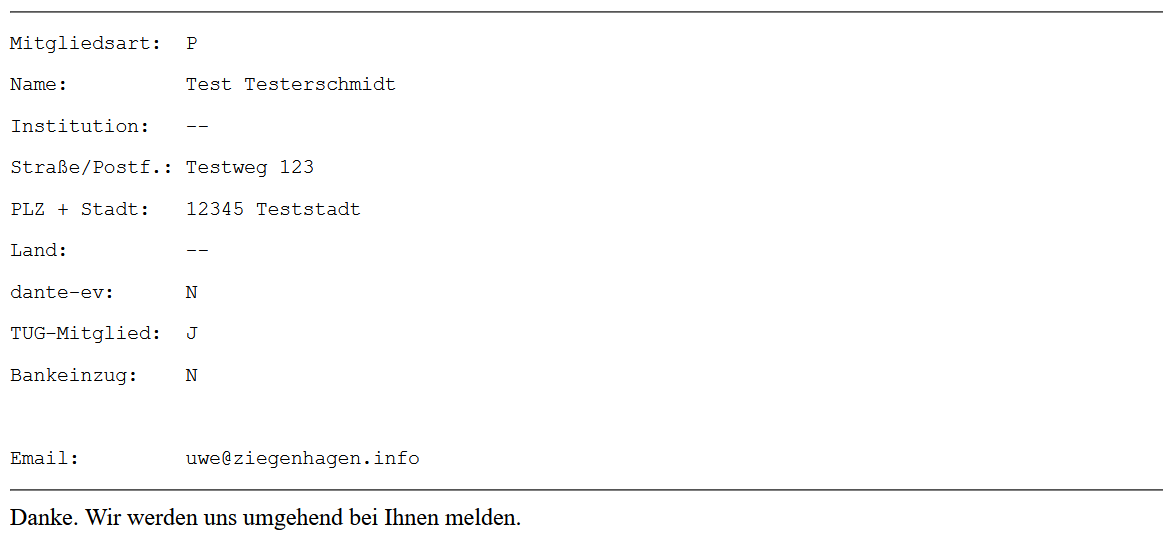
\includegraphics[width=\textwidth]{onlineform-antwort.png}}
\end{center}

\end{frame}

 \begin{frame}
\frametitle{Online Form at www.dante.de}

\begin{center}
\fbox{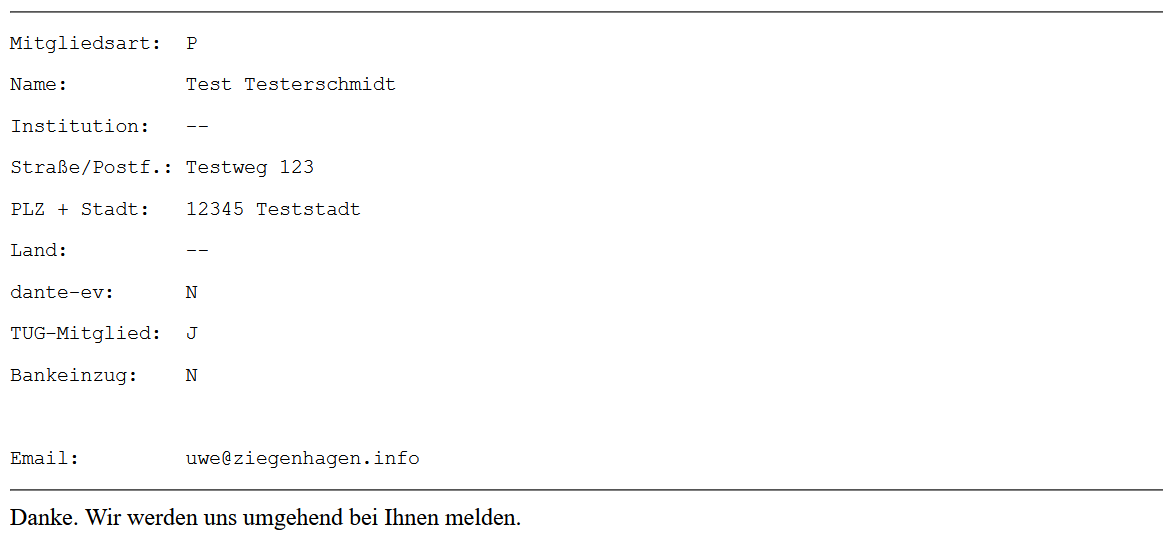
\includegraphics[width=\textwidth]{onlineform-antwort.png}}
\end{center}

\end{frame}

\begin{frame}[fragile]
\frametitle{Received E-Mail}

{\footnotesize
\begin{lstlisting}
Name:          Test Testerschmidt
Mitgliedsart:  P
Institution:   --
Strasse/Postf.: Testweg 123
PLZ:           12345
Stadt:         Teststadt
Land:          --

Email:   uwe@ziegenhagen.info 

dante-ev:      N
TUG-Mitglied:  J
Bankeinzug:    N
\end{lstlisting}
}

\textcolor{blue}{$\Rightarrow$ My answer depends on the membership type and the last three J/N values}

\end{frame}

\begin{frame}
\frametitle{Required Libraries}

\begin{description}
\item[toml] read PW from config file
\item[imaplib] read mails on server
\item[email] create e-mail objects from server replies
\item[traceback] to handle stack traces
\end{description}

Whole code is \enquote{hacky} and mostly the result of copy \& past, but it works\ldots
\end{frame}


\begin{frame}[fragile]
\frametitle{toml}

\begin{itemize}
	\item toml = \enquote{Tom’s Obvious Minimal Language}
	\item Simple way to store configuration settings in external files
	\item Much similar to ini files
\end{itemize}

\begin{lstlisting}[language={Python}]
import toml

settings = toml.load('settings.toml')
FROM_EMAIL = settings['myemail'] 
\end{lstlisting}

\end{frame}

\begin{frame}[fragile]
\frametitle{Helper Function}

Helper function to parse the mail

\begin{lstlisting}[language={Python},basicstyle={\footnotesize}]
def parse_mail(text):
    zeilen = text.split('\n') # create array
    daten = {} # empty dict

    for zeile in zeilen:
        splits = zeile.split(':')
        if len(splits) == 2:
            daten[splits[0].strip()] = splits[1].strip()
            
    return daten
\end{lstlisting}

\end{frame}

\begin{frame}
\frametitle{Reading mails from Gmail}

\begin{itemize}
\item the hacky copy \& paste part,  see the Python file in github
\item was quite a struggle: multipart-messages, base64, Ansi/ASCII/UTF8
\item latest updates:

\begin{itemize}
	\item filter interesting mails on the server (\texttt{mail.search()})
	\item trying to get rid of multipart code
\end{itemize}

\item Function returns array of all relevant mails

\end{itemize}
\end{frame}

\begin{frame}

\begin{center}
\hspace*{-1em}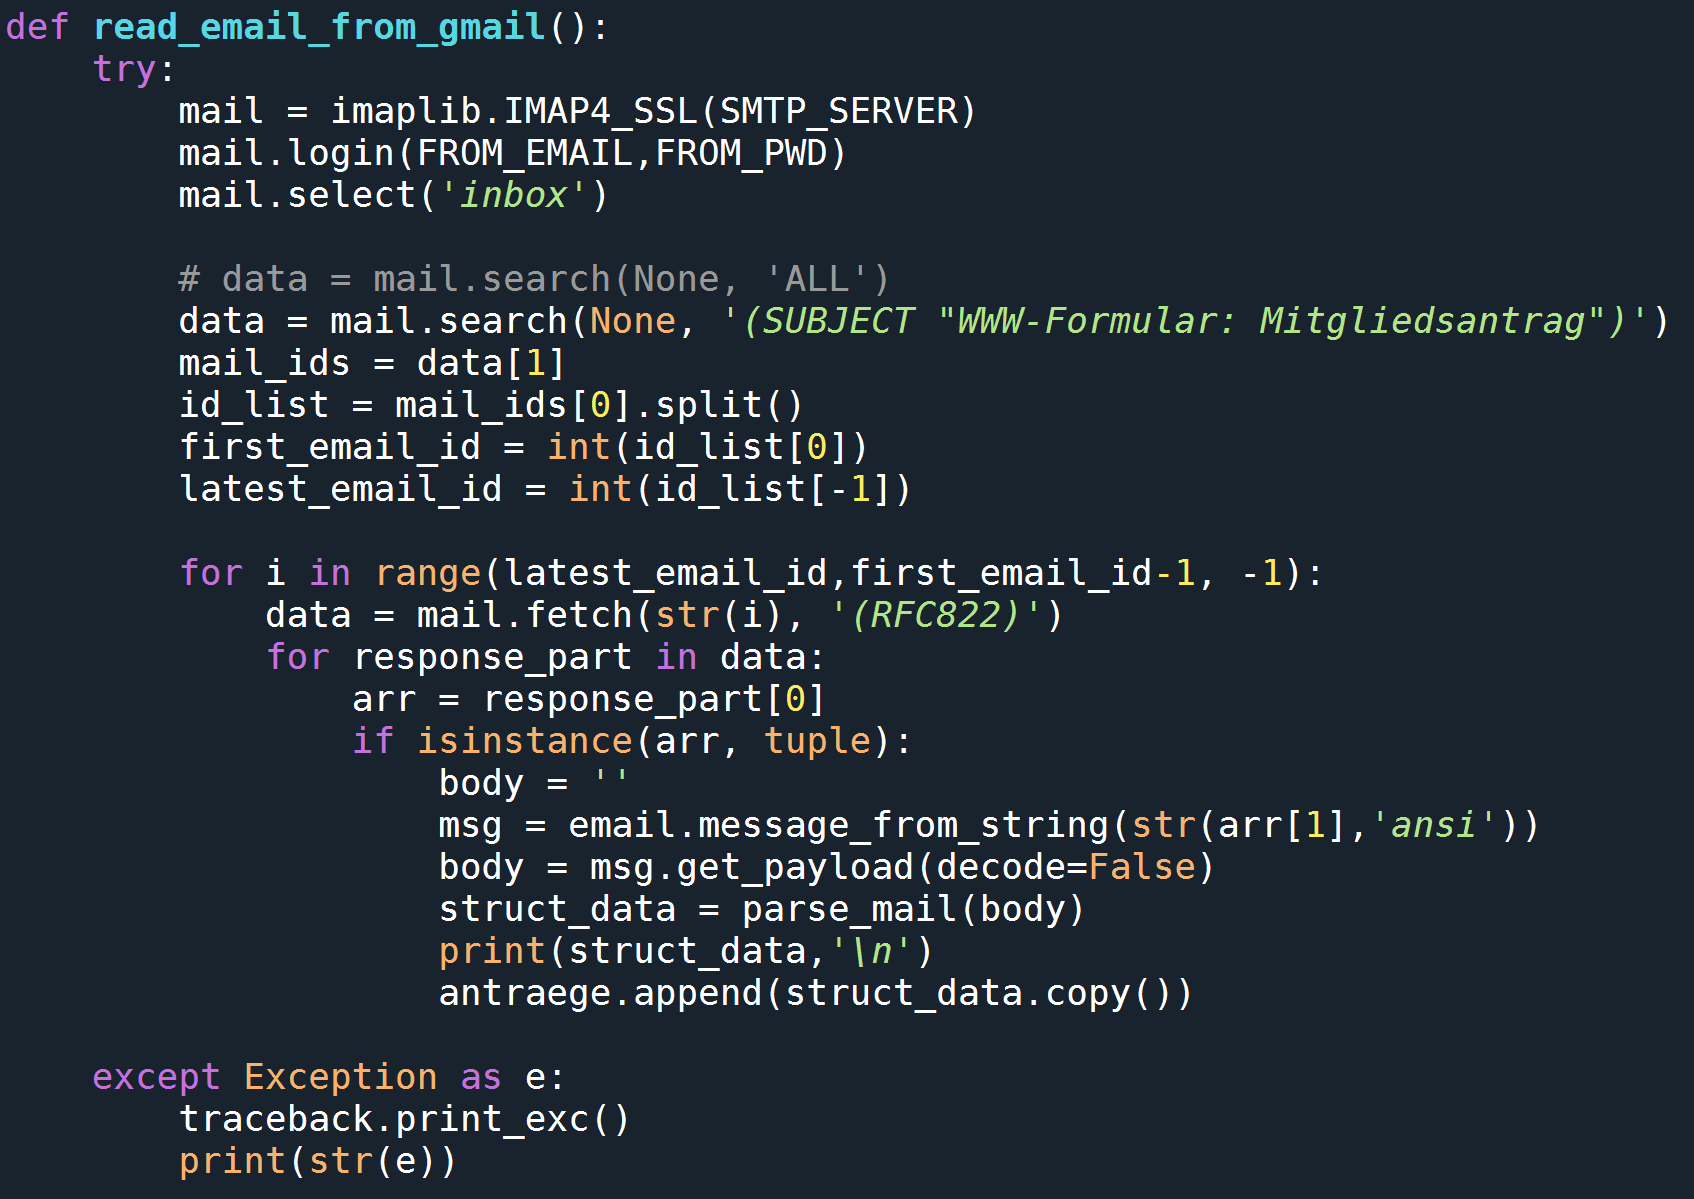
\includegraphics[width=1.1\textwidth]{readmails}
\end{center}

\end{frame}

\begin{frame}
\frametitle{Preparing answers}

\begin{itemize}
\item Pre-defined templates for different scenarios: pays him/herself, TUG-membership y/n, reduced fee, etc.
\item $\Rightarrow$ nasty if/elif/else statements in the \texttt{process\textunderscore mails} function
\item Templates are combined, replacements made, final text printed
\item No automated sending, yet, need to build \enquote{trust} in the code, rare scenarios not treated, yet.
\end{itemize}
\end{frame}

\begin{frame}
\frametitle{Preparing answers}

\begin{center}
\hspace*{-1em}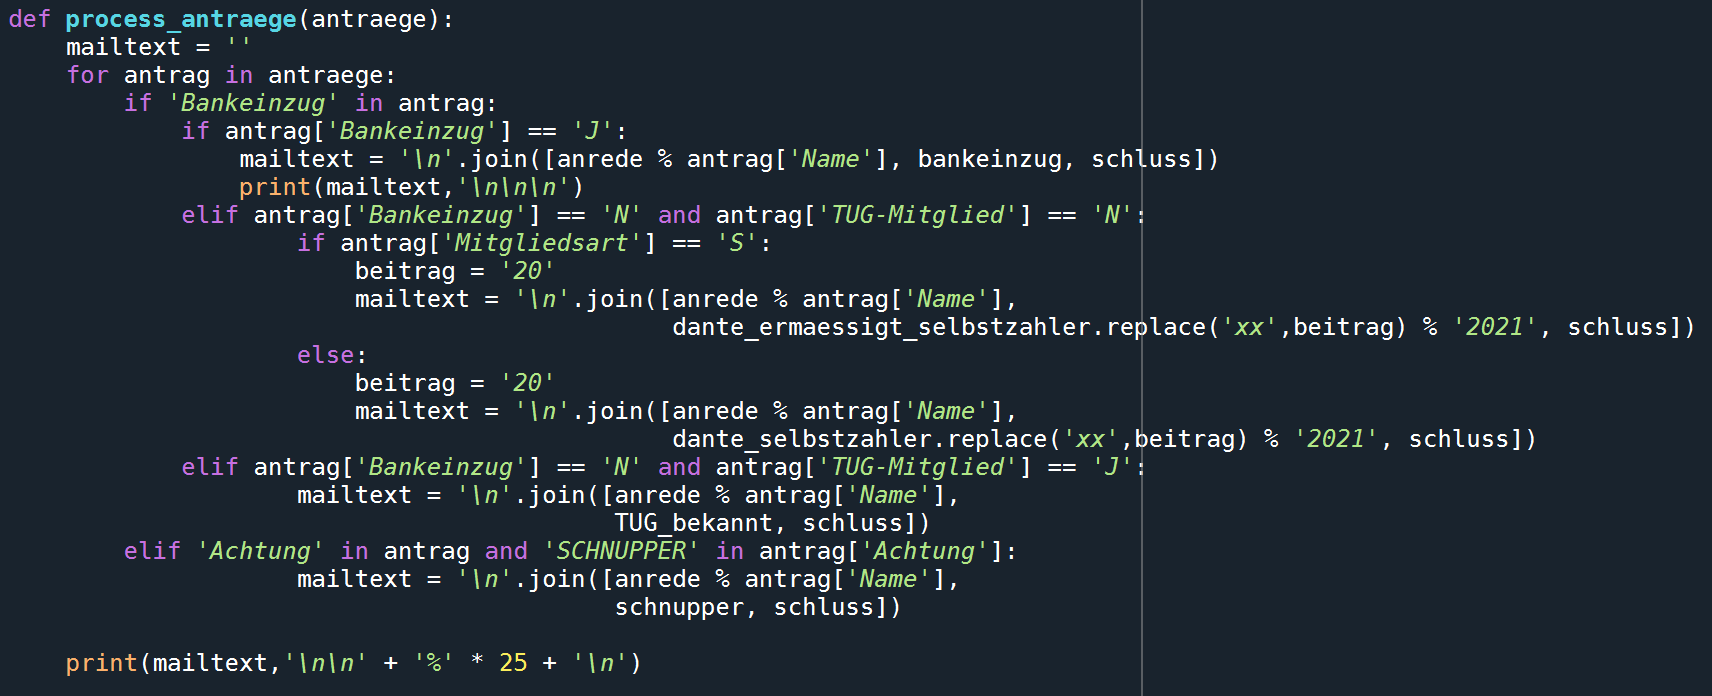
\includegraphics[width=1.1\textwidth]{process}
\end{center}

\end{frame}

\begin{frame}
\section{Managing Mailinglists}
\end{frame}

\begin{frame}
\frametitle{Mailinglists}

\begin{itemize}
\item Dante e.V. provides various public/semi-public mailing lists
\item SPAM is huge problem, some months ago: dozens of new signup-requests per day
\item $\Rightarrow$ Automation necessary $\Rightarrow$ Selenium
\item Selenium = web-testing framework, controls browser from Python
\end{itemize}
\end{frame}

\begin{frame}
\frametitle{Selenium 1}

\begin{itemize}
	\item load selenium packages
	\item defines the sites to be handled
	\item load passwords via toml
\end{itemize}

\begin{center}
\hspace*{-1em}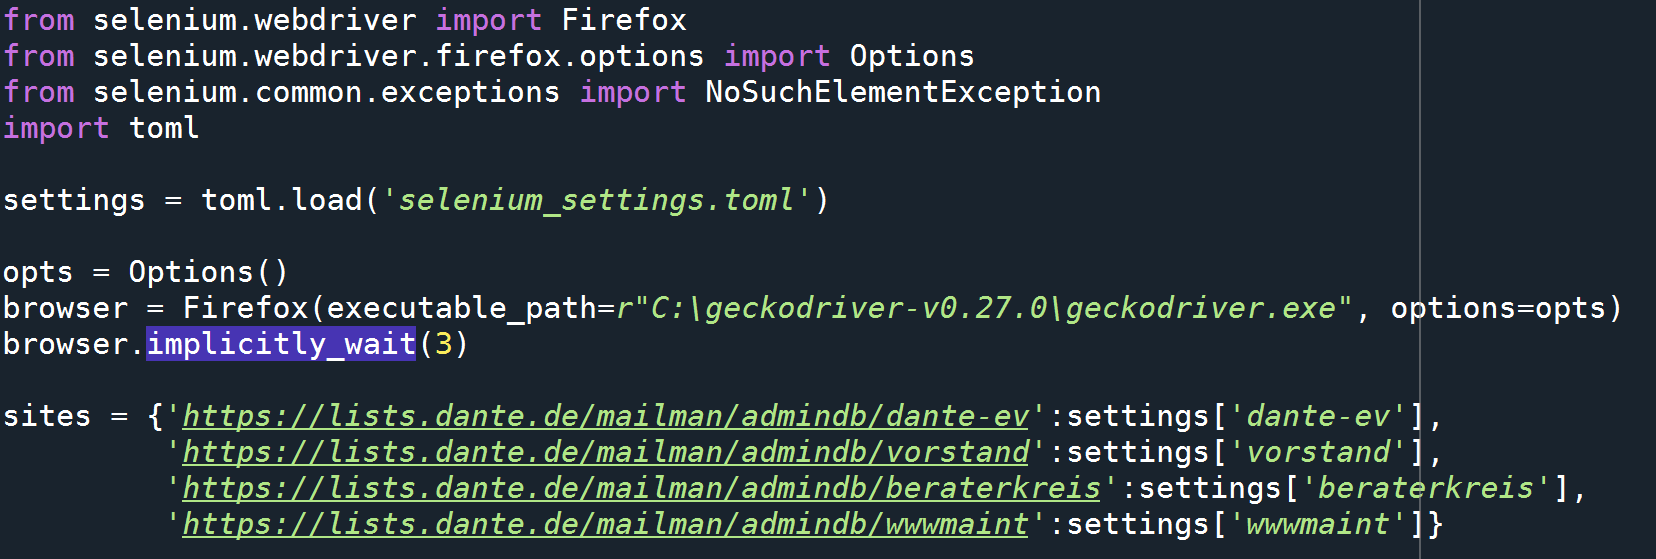
\includegraphics[width=1.1\textwidth]{sel1}
\end{center}

\end{frame}

\begin{frame}
\frametitle{Selenium 2}

\begin{itemize}
	\item login to each mailinglist
	\item enable deletion of all requests
	\item click submit button
\end{itemize}\vspace*{-1em}


\begin{center}
\hspace*{-1em}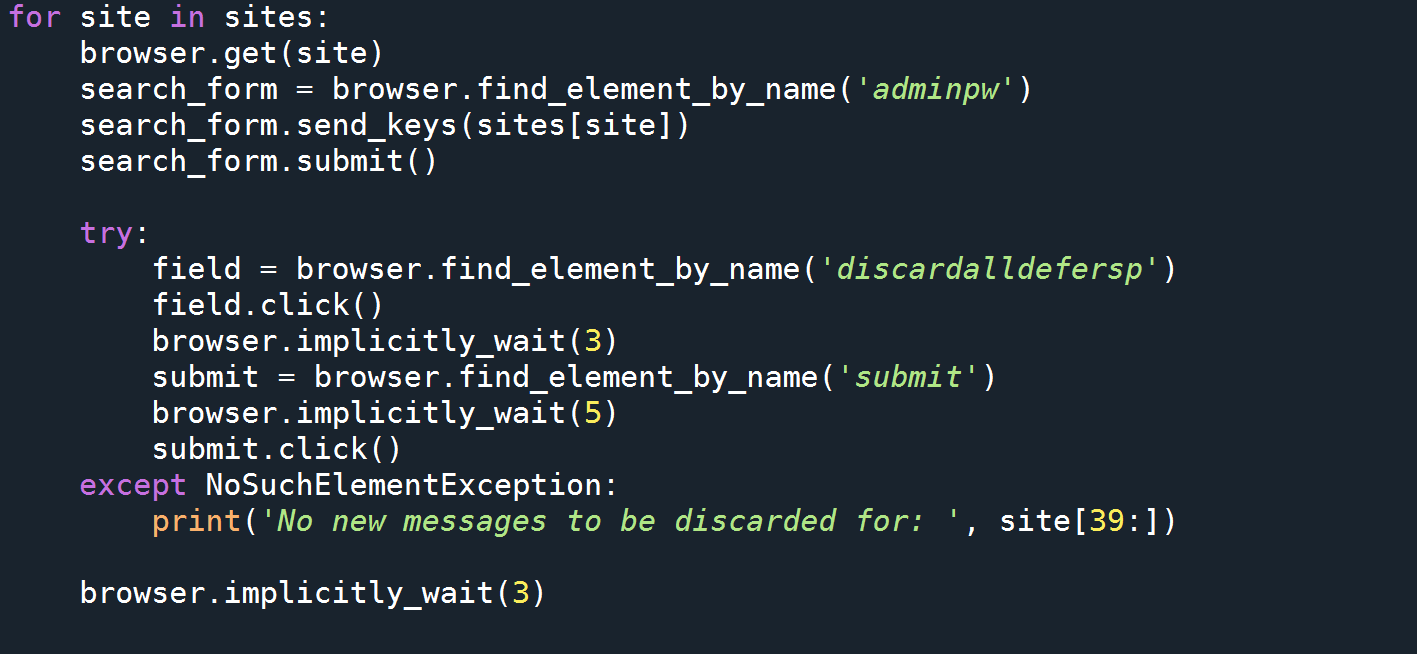
\includegraphics[width=1.1\textwidth]{sel2}
\end{center}

\end{frame}

\begin{frame}
\frametitle{Selenium 3}

\begin{itemize}
	\item ban all new-user requests if they do not contain \enquote{)}
\end{itemize}\vspace*{-1em}


\begin{center}
\hspace*{-1em}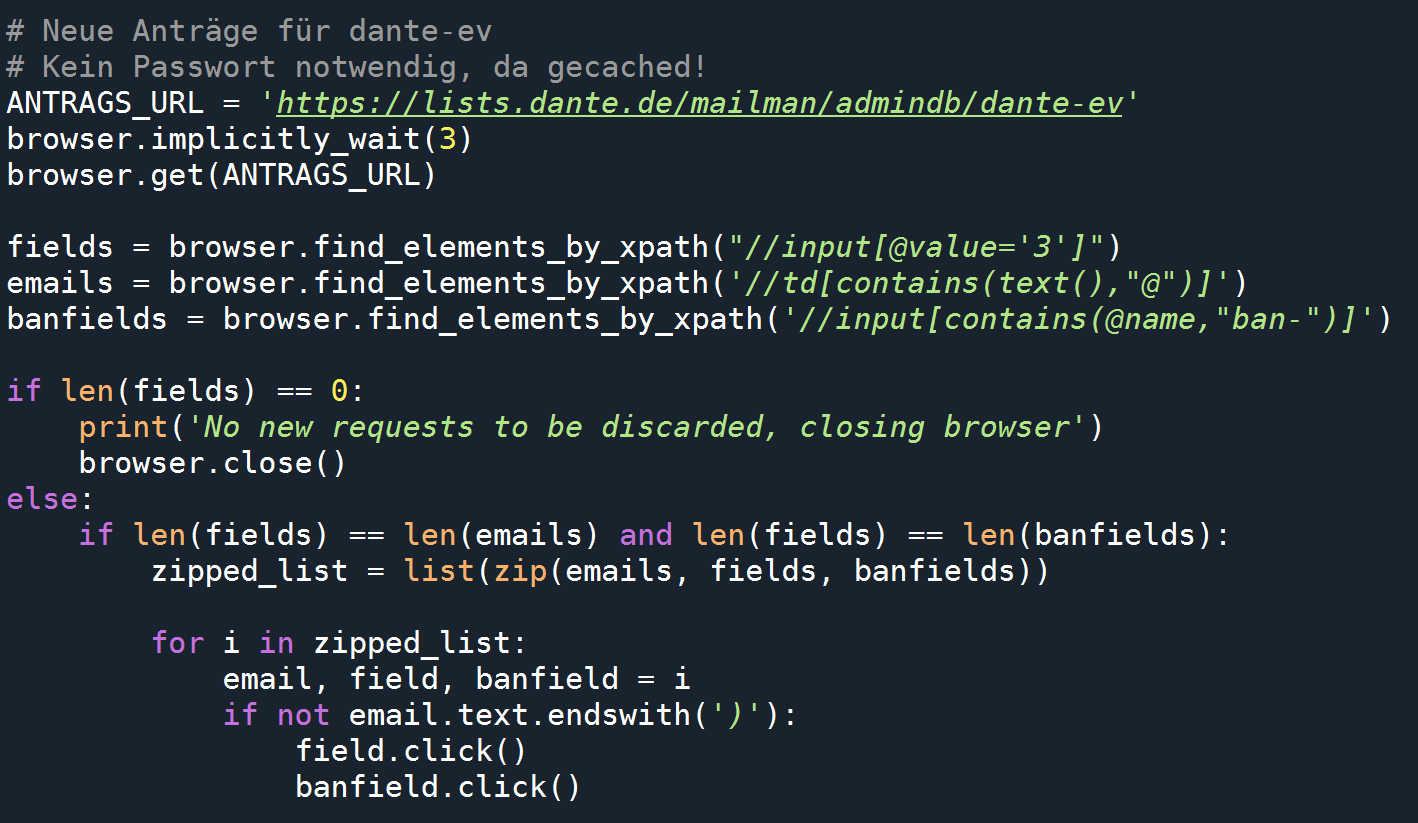
\includegraphics[width=1.1\textwidth]{sel3}
\end{center}

\end{frame}


\end{document}